\chapter{Systemy operacyjne}

Materiały teoretyczne zostały opracowane na podstawie slajdów Marcina Engela i Marcina Peczarskiego. \quad \textbf{\red{(przyp. red.: potrzebny link do źródła)}}

\section*{Podstawa programowa}
\begin{enumerate}
    \item \textbf{Mechanizmy sprzętowe} potrzebne do realizacji wielodostępnych, wieloprocesorowych systemów operacyjnych.
    \item Podstawy \textbf{programowania niskopoziomowego}, asembler.
    \item Algorytmy \textbf{szeregowania procesów}.
    \item \textbf{Pamięć wirtualna}. Cechy charakterystyczne różnych technik realizacji pamięci wirtualnej.
    \item Funkcje systemowe do \textbf{obsługi plików} z poziomu użytkownika (czynności wykonywane przez system operacyjny, struktury danych).
\end{enumerate}

\section{Programowanie niskopoziomowe}

Przypomnienie assemblera: w składni NASM operandy są w kolejności najpierw \textbf{dest} (miejsce docelowe) później \textbf{src} (źródło).

\begin{example}
    Instrukcja \;
    \verb|mov ax, 9| \;
    zapisuje wartość 9 do rejestru ax.
\end{example}

\subsection{Reprezentacja liczb całkowitych}
Wartość $n$-bitową $b_{n - 1} b_{n - 2} \dots b_1 b_0$ w \textbf{naturalnym kodzie binarnym} (NKB) 
interpretujemy jako $\sum_{i = 0}^{n - 1} b_i 2^i$, a w \textbf{kodzie uzupełnieniowym do dwójki} (U2) jako $-b_{n-1} 2^{n - 1} + \sum_{i = 0}^{n - 2} b_i 2^i$.

Te same układy arytmetyczne mogą być użyte do dodawania, odejmowania i mnożenia w NKB i U2, niezależnie od interpretacji.

\textbf{Little-endian} (cienkokońcowość) to forma zapisu danych, w której najmniej znaczący bajt umieszczany jest jako pierwszy. W \textbf{big-endian} (grubokońcowość) najbardziej znaczący bajt umieszczony jest jako pierwszy.

Procesory x86 używają little-endian.

% TODO
\begin{editorsnote}
    Brakuje interpretacji moduł-znak, warto o niej tu coś napisać, bo pojawia się w dalszej teorii i zadaniach.
\end{editorsnote}

\begin{exam}
    W ośmiobitowym rejestrze procesora zapisana jest wartość $(11000000)_2$, która interpretowana
    \answers
    {w naturalnym kodzie binarnym reprezentuje liczbę 192}
    {w kodzie uzupełnieniowym do dwójki reprezentuje liczbę $-64$}
    {w kodzie moduł-znak reprezentuje liczbę $-64$}
    \bigskip

    \begin{enumerate}[\bf A.]
        \item Liczby w naturalnym kodzie binarnym są interpretowane jako $\sum_{i = 0}^{n - 1} b_i 2^i$, zatem wartość $(11000000)_2$ reprezentuje liczbę $2^7 + 2^6 = 192$.

        \item Liczby w kodzie uzupełnieniowym do dwójki są interpretowane jako $-b_{n-1} 2^{n - 1} + \sum_{i = 0}^{n - 2} b_i 2^i$, zatem wartość $(11000000)_2$ reprezentuje liczbę $-2^7 + 2^6 = -64$.

        \item Liczby w kodzie moduł-znak są interpretowane jako $(-1)^{b_{n-1}} \cdot \sum_{i = 0}^{n - 2} b_i 2^i$, zatem wartość $(11000000)_2$ reprezentuje liczbę $(-1) \cdot (2^6) = -64$.
    \end{enumerate}
\end{exam}

\subsection{Rejestr stanu}

W x86 obecny jest rejestr stanu. Zawiera on pewne bity, aktualizowane po każdej operacji arytmetyczno-logicznej. Ważniejsze bity:
\begin{itemize}
    \item bit {\ttfamily OF} -- \textit{overflow}, wynik spoza zakresu przy interpretacji U2,
    \item bit {\ttfamily SF} -- \textit{sign}, najstarszy bit wyniku operacji, przy interpretacji w U2 znak wyniku,
    \item bit {\ttfamily CF}  -- \textit{carry}, przeniesienie lub pożyczka z najstarszego bitu,
    \item bit {\ttfamily ZF} -- \textit{zero}, wynik operacji jest zerem.
\end{itemize}

\begin{example}
    \begin{tabular}{r r r}
        \hline
        odejmowanie & interpretacja w NKB & interpretacja w U2 \\
        \hline
        10000010 & 130 & -126 \\
        00000011 & 3 & 3\\
        \hline
        01111111 & 127 & 127 \\ 
        \hline
    \end{tabular}

    Bity stanu: \;
    {\ttfamily CF} $ = 0$ \; 
    {\ttfamily OF} $ = 1$ \; 
    {\ttfamily SF} $ = 0$ \; 

    \vspace{8pt}
    \begin{tabular}{r r r}
        \hline
        odejmowanie & interpretacja w NKB & interpretacja w U2 \\
        \hline
        10000001 & 129 & -127 \\
        10000010 & 130 & -126 \\
        \hline
        11111111 & 255 & -1 \\ 
        \hline
    \end{tabular}

    Bity stanu: \;
    {\ttfamily CF} $ = 1$ \; 
    {\ttfamily OF} $ = 0$ \; 
    {\ttfamily SF} $ = 1$ \; 
\end{example}

\subsection{Architektury}

\begin{tabular}{|p{8cm}|p{8cm}|}
    \hline
    \textbf{CISC} (Complex Instruction Set Computer) & 
    \textbf{RISC} (Reduced Instruction Set Computer) \\
    \hline
    wiele rozkazów, potencjalnie skomplikowanych & ograniczony, proste rozkazy \\
    \hline
    mała liczba rejestrów lub rejestry specjalizowane & duża liczba uniwersalnych rejestrów \\
    \hline
    rozkazy arytmetyczno-logiczne pobierają argumenty z pamięci lub umieszają w niej wynik & rozkazy arytmetyczno-logiczne wykonywane są tylko na rejestrach \\
    \hline
    duża liczba trybów adresowania & mała liczba trybów adresowania \\
    \hline
    dozwolone adresowanie niewyrównane & dozwolone tylko adresowanie wyrównane \\
    \hline
    kody rozkazów zmiennej długości, od jednego do kilkunastu bajtów &
    kody rozkazów o stałej długości, typowo 4 bajty \\
    \hline
    prefiksowanie rozkazów, utrudniające dekodowanie &
    stałe rozmieszczenie pól w kodach, ułatwiające dekodowanie \\
    \hline
    przykładem jest x86, często używane w PC
    & przykładem jest ARM, często używane w smartfonach i Mac'ach \\
    \hline
\end{tabular}

\subsection{Potokowanie}
Różne części hardware'u są odpowiedzialne za kolejne fazy przetwarzania instrukcji. Można zatem równolegle przetwarzać kolejne instrukcje, potencjalnie znacznie przyspieszając działanie.

\begin{figure}[H]
    \centering
    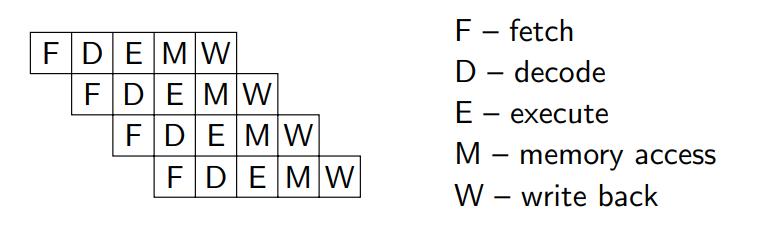
\includegraphics[scale=0.35]{rozdziały/images/SO/potokowanie.png}
    \caption{Fazy przetwarzania instrukcji w czasie.}
\end{figure}

Przy skokach warunkowych, nie wiadomo jakie instrukcje zaczynać przetwarzać do przodu. Współczesne procesory dokonują predykcji skoków.

Rozkazy x86 źle się potokuje, bo kod rozkazu nie ma stałego rozmiaru, jest bardziej skomplikowany, oraz czasy wykonywania poszczególnych rozkazów mogą się bardzo różnić. 

Rozwiązanie: pośrednie tłumaczenie rozkazów na RISC.

\begin{problems}
    \prob W procesorze x86 wykonano następujące instrukcje:
    \begin{gas}
        mov al, 3
        mov bl, 130
        sub al, bl
    \end{gas}
    Wtedy
    \answers{w rejestrze \gasinline{al} jest zapisana wartość $-127$ przy interpretacji w kodzie uzupełnień do dwóch}{w rejestrze \gasinline{al} jest zapisana wartość $127$ przy interpretacji w naturalnym kodzie binarnym}{ustawione zostaną flagi CF, OF, SF}

    \prob Cechą architektury RISC jest
    \answers{zapisywanie wyników instrukcji arytmetyczno-logicznych tylko w rejestrach}{kodowanie wszystkich instrukcji maszynowych za pomocą tej samej liczby bajtów}{dopuszczenie adresowania niewyrównanego}

    \prob Cechą architektury CISC jest
    \answers
    {zapisywanie wyników instrukcji arytmetyczno-logicznych tylko w rejestrach}
    {kodowanie wszystkich instrukcji maszynowych za pomocą tej samej liczby bajtów}
    {dopuszczenie adresowania niewyrównanego}

    \prob W czterech kolejnych bajtach pamięci, począwszy od adresu $X$, znajdują się odpowiednio wartości 1, 3, 5 i 7. Procesor cienkokońcówkowy (ang. \textit{little-endian}) wczytał 32-bitową liczbę spod adresu $X$, odjął od niej $(16)_{10}$ i zapisał wynik pod adresem $X$. Po tych operacjach bajt o adresie
    \answers{$X$ zawiera wartość $(F1)_{16}$}{$X+1$ zawiera wartość $(03)_{16}$}{$X+2$ zawiera wartość $(05)_{16}$}

    \prob W ośmiobitowym rejestrze procesora zapisana jest wartość $(11000000)_2$, która interpretowana
    \answers
    {w naturalnym kodzie binarnym reprezentuje liczbę 192}
    {w kodzie uzupełnieniowym do dwójki reprezentuje liczbę $-64$}
    {w kodzie moduł-znak reprezentuje liczbę $-64$}

    \prob Przetwarzanie potokowe
    \answers{zawsze przyspiesza lub nie spowalnia wykonywania rozkazów}{niewykorzystywane jest dla rozkazu skoku}{zostało zastosowane po raz pierwszy w procesorach Pentium}

    % TODO
    \textbf{\red{(przyp. red.: odpowiedzi C. nie da się wywnioskować na podstawie części teoretycznej)}}

    \prob Każdy procesor 32-bitowy ma
    \answers
    {32-bitową zewnętrzną szynę danych}
    {32-bitową zewnętrzną szynę adresową}
    {32-bitowe rejestry danych}
    
    % TODO
    \textbf{\red{(przyp. red.: tego zadania nie da się wywnioskować na podstawie części teoretycznej)}}
\end{problems} 

\section{Szeregowanie procesów}

\textbf{Program} to zestaw instrukcji w formie kodu, tekstu.

\textbf{Proces} to wykonanie programu. Aktywny obiekt w odróżnieniu od programu. Wiele procesów może wykonywać ten sam program ale proces wykonuje tylko jeden na raz. Proces może w trakcie działania zmienić wykonywany program. 

Na proces składają się: 

\begin{itemize}
    \item przydzielona mu pamięć, czyli \textbf{przestrzeń adresowa} (zawiera między innymi Kod programu, dane programu, stos procesu)
    \item zbiór rejestrów (licznik rozkazów, wskaźnik stosu, rejestr stanu, rejestry specjalne)
    \item informacje administracyjne (stan, kod zakończenia, ...)
    \item inne zasoby potrzebne do wykonywania programu:
        \begin{itemize}
            \item otwarte pliki
            \item identyfikator procesu (pid)
            \item przestrzeń wejścia-wyjścia
            \item stosy alternatywne (wykorzystywane w trakcie obsługi przerwań lub wywołań systemowych)
        \end{itemize}
\end{itemize}

Informacje o procesach w systemie przechowywane są w tablicy/liście procesów w formie PCB (Process Control Block). Na PCB składają kluczowe dane do działania procesów.

\textbf{Podział czasu}:
\begin{itemize}
    \item każdy proces otrzymuje kwant czasu
    \item po upływie kwantu procesor "odkłada" wykonanie procesu i rozpoczyna wykonanie innego - \textbf{przełączanie kontekstu}
    \item proces nie musi wykorzystywać całego kwantu czasu (np. wykonanie operacji wejścia-wyjścia)
\end{itemize}    

\textbf{Przełączanie kontekstu}
\begin{center}
    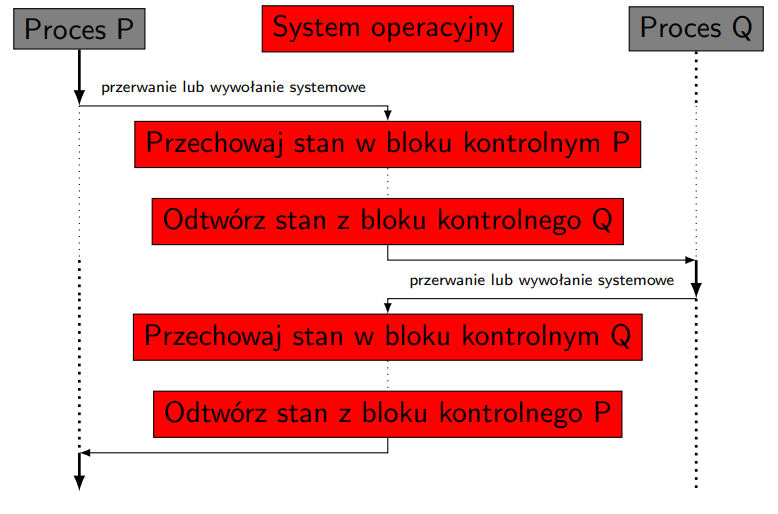
\includegraphics[scale=0.35]{rozdziały/images/SO/context_switching.png}
\end{center}

\textbf{Szeregowanie} to zadanie wyboru kolejnego procesu:
\begin{itemize}
    \item do wykonania (szeregowanie krótkoterminowe)
    \item do wprowadzenia do systemu (szeregowanie długoterminowe). 
        \begin{itemize}
            \item Outdated, dotyczyło raczej systemów z przetwarzaniem wsadowym.
            \item Chodziło o dobranie procesów tak, aby procesor był równomiernie wykorzystywany. Stworzenie mieszanki procesów ograniczanych przez wejście/wyjście i obliczeniowych. 
        \end{itemize}
\end{itemize}

\subsection{Szeregowanie krótkoterminowe}
    \subsubsection{Uproszczony schemat stanów procesów}   
        \begin{center}
            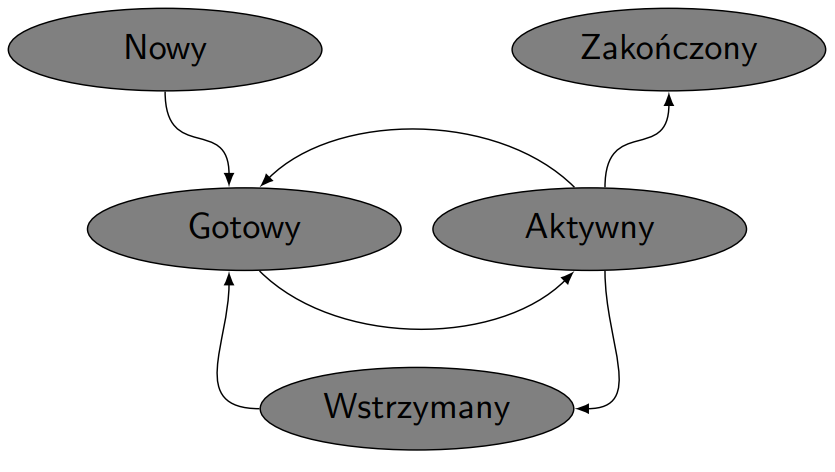
\includegraphics[scale=0.3]{rozdziały/images/SO/stany_procesu.png}
        \end{center}


    Szeregowanie krótkoterminowe można podzielić na 2 typy:
    \begin{itemize}
        \item \textbf{wywłaszczające}. Decyzja o przydziale procesora, gdy:
            \begin{itemize}
                \item aktywny proces zmienia stan na wstrzymany 
                \\ (dobrowolne oddanie procesora: operacja wejścia/wyjścia, wstrzymanie na semaforze)
                \item aktywny proces zmienia stan na gotowy (w systemie z podziałem czasu kończy się kwant czasu)
                \item wstrzymany lub nowy proces zmienia stan na gotowy
                \\ (wstrzymany $\rightarrow$ gotowy, np. system otrzymuje przerwanie o zakończeniu operacji wejścia/wyjścia)
                \item aktywny proces kończy się 
            \end{itemize}
        \item \textbf{niewywłaszczające} Decyzja o przydziale procesora, gdy:
            \begin{itemize}
                \item aktywny proces zmienia stan na wstrzymany
                \item aktywny proces kończy się 
            \end{itemize}
    \end{itemize}

    \subsubsection{Szeregowanie niewywłaszczające}
        W ogólności mało przydatne, jednak jedyna metoda w przypadku niektórych sprzętów (np. tych bez wsparcia systemowego w postaci czasomierza). Występuje mniej problemów synchronizacyjnych, jednak procesy dłużej oczekują na możliwość wykonania się.
    \subsubsection{Szeregowanie wywłaszczające}
        Synchronizacja dostępu do danych dzielonych jest wymagana (semafory, monitory). Ponownie można tutaj wprowadzić podział:
        \begin{itemize}
            \item jądro wywłaszczalne - przełączamy kontekst nawet w trakcie wykonywania procedur jądra systemowego
            \item jądro niewywłaszczalne - wszystko można przełączyć oprócz procedur jądra systemu (czekamy, aż ona się skończy)
        \end{itemize} 
\subsection{Algorytmy szeregowania}
    \subsubsection{FCFS}
    \textbf{F}irst \textbf{C}ome \textbf{F}irst-\textbf{S}erved - szeregowanie niewywłaszczające na zasadzie kolejki prostej. Przychodzące procesy na koniec kolejki, następne do wykonania bierzemy z jej początku.
    \\ \\

    Przykład 1.
    \begin{figure}[!htb]
       \begin{minipage}{0.15\textwidth}
         \centering
         Procesy
         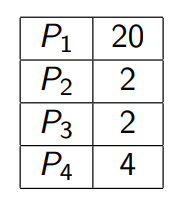
\includegraphics[scale=0.35]{rozdziały/images/SO/FCFS_procesy1.png}
       \end{minipage}\hfill
       \begin{minipage}{0.5\textwidth}
         \centering
         Jeśli kolejność w kolejce to $P_1$, $P_2$, $P_3$, $P_4$
         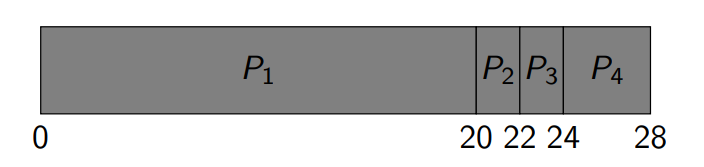
\includegraphics[scale=0.3]{rozdziały/images/SO/FCFS_kolejnosc1.png}
       \end{minipage}\hfill
        \begin{minipage}{0.3\textwidth}
            \centering
            Czasy oczekiwania:
            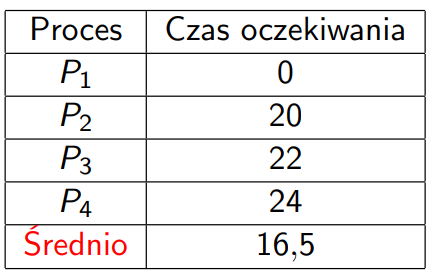
\includegraphics[scale=0.25]{rozdziały/images/SO/FCFS_czasowo1.png}
        \end{minipage}
    \end{figure}


    Przykład 2.
    \begin{figure}[!htb]
       \begin{minipage}{0.15\textwidth}
         \centering
         Procesy
         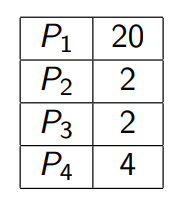
\includegraphics[scale=0.35]{rozdziały/images/SO/FCFS_procesy1.png}
       \end{minipage}\hfill
       \begin{minipage}{0.5\textwidth}
         \centering
         Jeśli kolejność w kolejce to $P_4$, $P_3$, $P_2$, $P_1$
         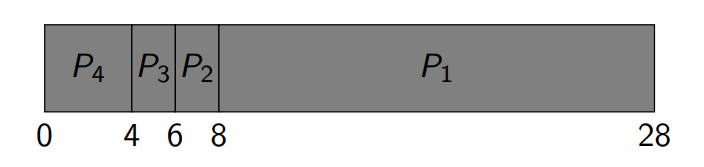
\includegraphics[scale=0.3]{rozdziały/images/SO/FCFS_kolejnosc2.png}
       \end{minipage}\hfill
        \begin{minipage}{0.3\textwidth}
            \centering
            Czasy oczekiwania:
            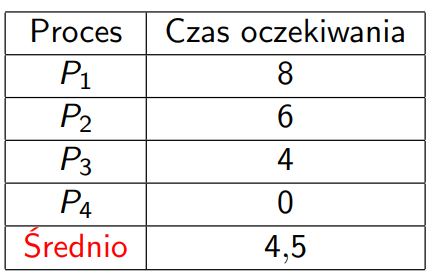
\includegraphics[scale=0.25]{rozdziały/images/SO/FCFS_czasowo2.png}
        \end{minipage}
    \end{figure}

    Wnioski:    
    \begin{itemize}
        \item Łatwy do zrozumienia i zaimplementowania
        \item Średni czas oczekiwania może być długi
        \item Duża wariancja czasu oczekiwania
        \item Efekt konwoju - proces $P_1$ wykonujący 1 sekundowe fazy aktywności. Procesy $P_2 \ldots P_n$ wykonujące 1200 operacji wyjścia i wyjścia. Skutek: $P_2\ldots P_n$ szybko wykorzystają swoją fazę i będą musiały czekać na kolejną 1200 razy, co daje czas oczekiwania $1200s = 20m$
    \end{itemize}

\subsubsection{SJF}
    \textbf{S}hortest \textbf{J}ob \textbf{F}irst - szeregowanie niewywłaszczające. Algorytm zachłanny, optymalizujący średni czas oczekiwania. Czas wykonania jednak w ogólności nie jest znany, dlatego stosuje się heurystyki. Najpierw bierzemy procesy o najkrótszej fazie. \\ 
    
    Przykład:
    \begin{figure}[!htb]
       \begin{minipage}{0.15\textwidth}
         \centering
         Procesy
         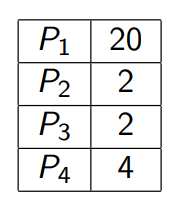
\includegraphics[scale=0.35]{rozdziały/images/SO/SJF_procesy.png}
       \end{minipage}\hfill
       \begin{minipage}{0.5\textwidth}
         \centering
         Przydział procesora
         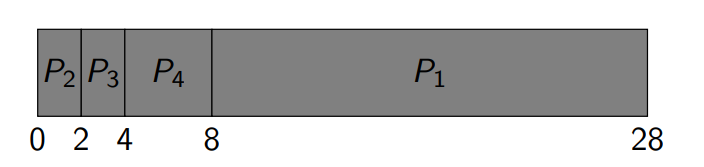
\includegraphics[scale=0.3]{rozdziały/images/SO/SJF_kolejnosc1.png}
       \end{minipage}\hfill
        \begin{minipage}{0.3\textwidth}
            \centering
            Czasy oczekiwania:
            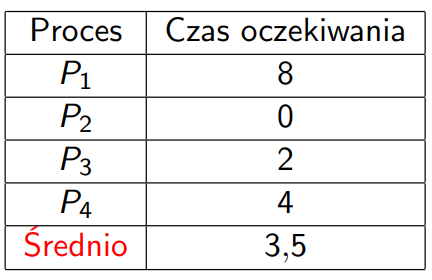
\includegraphics[scale=0.25]{rozdziały/images/SO/SJF_czasowo.png}
        \end{minipage}
    \end{figure}

    Wnioski:
    \begin{itemize}
        \item Optymalizuje średni czas oczekiwania
        \item Nie daje się zastosować przy planowaniu przydziału procesora, bo trudno oszacować długość następnej fazy procesora
    \end{itemize}

    
\subsubsection{SRTF}
    SRTF - \textbf{S}hortest \textbf{R}emaining \textbf{T}ime \textbf{F}irst. Wywłaszczająca wersja \textbf{SJF} - gdy pojawia się nowy proces o krótszej fazie procesora niż długość fazy pozostałej wykonywanemu, to dochodzi do wywłaszczenia. \\

    Przykład:
    \begin{figure}[!htb]
       \begin{minipage}{0.3\textwidth}
         \centering
         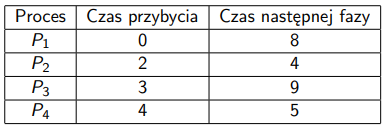
\includegraphics[scale=0.5]{rozdziały/images/SO/srtf_procesy.png}
       \end{minipage}\hfill
       \begin{minipage}{0.5\textwidth}
         \centering
         Przydział procesora
         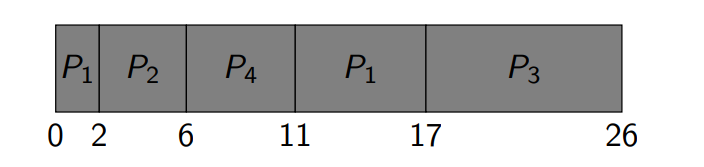
\includegraphics[scale=0.3]{rozdziały/images/SO/SRTF_kolejnosc1.png}
       \end{minipage}
    \end{figure}

    Wnioski:
    \begin{itemize}
        \item Może wystąpić zagłodzenie
    \end{itemize}

\subsubsection{Szeregowanie priorytetowe}
    Szeregowanie priorytetowe to uogólniona wersja \textbf{SJF}. Priorytety mogą być:
    \begin{itemize}
        \item wewnętrzne - obliczane przez SO na podstawie pewnych właściwości procesu
        \item zewnętrzne - przydzielane poza SO
    \end{itemize} 

    Wnioski:
    \begin{itemize}
        \item Może wystąpić zagłodzenie
        \item Może być wywłaszczające lub niewywłaszczające
    \end{itemize}

    Można sobie jednak radzić z zagłodzeniem co jakiś czas zwiększając priorytet procesom niewybranym do wykonania - \textbf{postarzanie}.
    

\subsubsection{Szeregowanie rotacyjne}
    Round-robin (RR) - wywłaszczająca wersja FCFS. Procesy gotowe przechowywane są w kolejce. Wykonywany proces jest wywłaszczany co ustalony kwant czasu i wraca na koniec kolejki. Do wykonania wybierany jest następny proces z kolejki. \\

    Przykład:
    \begin{figure}[!htb]
        \begin{minipage}{0.2\textwidth}
            \centering
            Procesy
            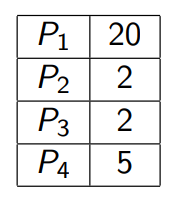
\includegraphics[scale=0.35]{rozdziały/images/SO/roundrobin_procesy.png}
        \end{minipage}\hfill
        \begin{minipage}{0.7\textwidth}
            \centering
            Przydział procesora \textbf{z kwantem czasu:} 3
            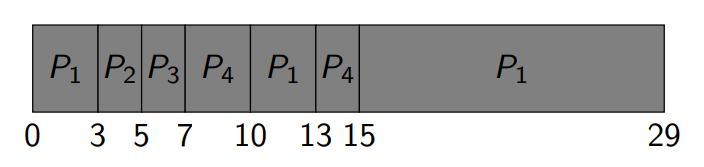
\includegraphics[scale=0.3]{rozdziały/images/SO/roundrobin_kolejnosc1.png}
        \end{minipage}
    \end{figure}

    Wnioski:
    \begin{itemize}
        \item Do realizacji konieczne wsparcie sprzętowe – czasomierz generujący przerwania
        \item Trzeba dobrze dobrać kwant czasu:
            \begin{itemize}
                \item Duży kwant czasu \textbf{RR}$=$\textbf{FCFS}
                \item Kwant czasu mniejszy od przełączania kontekstu $\rightarrow$ niewykorzystywany procesor.
            \end{itemize}
    \end{itemize}
    
    Szczególnym przypadkiem szeregowania rotacyjnego jest Podział Czasu - uzyskujemy je w momencie gdy kwant czasu wynosi $\varepsilon$ \\

    Przykład:
    \begin{figure}[!htb]
        \begin{minipage}{0.2\textwidth}
            \centering
            Procesy
            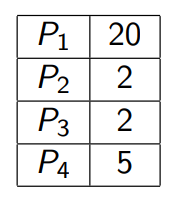
\includegraphics[scale=0.35]{rozdziały/images/SO/roundrobin_procesy.png}
        \end{minipage}\hfill
        \begin{minipage}{0.7\textwidth}
            \centering
            Przydział procesora \textbf{z kwantem czasu: $\varepsilon$}
            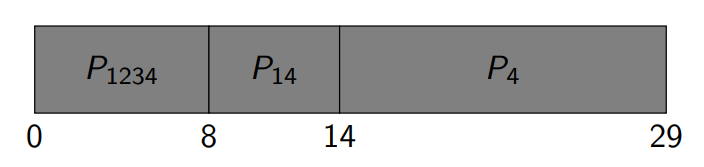
\includegraphics[scale=0.3]{rozdziały/images/SO/roundrobin_podzialczasu_kolejnosc1.png}
        \end{minipage}
    \end{figure}

\subsubsection{Szeregowanie wielopoziomowe}
Implementowane we współczesnych systemach, między innymi: Minix i Linux
\begin{itemize}
    \item Osobne kolejki dla poszczególnych grup procesów, np. 
        \begin{itemize}
        \item procesy czasu rzeczywistego
        \item procesy systemowe
        \item pierwszoplanowe procesy interakcyjne
        \item procesy drugoplanowe
        \end{itemize}
    \item Każda kolejka z własnym algorytmem szeregowania, np.
        \begin{itemize}
        \item pierwszoplanowe procesy interakcyjne – RR
        \item procesy drugoplanowe – FCFS
        \end{itemize}
    \item Zasady wyboru kolejki, np.
        \begin{itemize}
        \item procesy systemowe mają zawsze priorytet przed interakcyjnymi 
        \item kolejka procesów systemowych otrzymuje 80\% czasu procesora
        \end{itemize}
    \end{itemize}

\subsection{Systemy czasu rzeczywistego i ich szeregowanie}

\textbf{System reaktywny} to system działający w sposób ciągły. Otrzymuje dane wejściowe od układów sprzętowych i przetwarza i przekazuje innym. \\

\textbf{System czasu rzeczywistego} to system reaktywny, który musi spełniać ścisłe wymagania na czas reakcji. \\

\textbf{System wbudowany} to system, w którym komputer jest tylko jednym z wielu elementów, np. systemy sterujące lotem. \\


Szeregując systemy czasu rzeczywistego chcemy:
\begin{itemize}
    \item Zapewnić dotrzymania terminów uruchomienia poszczególnych procesów  (żeby piec nie wybuchł sobie, jak za późno świeczkę zgasimy).
    \item Zapewnić przewidywalność i powtarzalność
\end{itemize}

Szeregowanie systemów rzeczywistych można podzielić na:
\begin{itemize}
    \item Szeregowanie synchroniczne.
    \item Szeregowanie asynchroniczne.
\end{itemize}

\subsubsection{Szeregowanie synchroniczne}
    Czas procesora dzielimy na przedziały o ustalonej długości – \textbf{ramy} (frames). Program dzielimy na zadania. Zadania muszą kończyć się w ciągu jednej ramy. Opisywane za pomocą \textbf{tablicy szeregującej}, która zawiera przypisanie zadań do ram. Jest ona konstruowana \textit{a'priori}. \\ 
    
    Przykład (wg Ben-Ariego):
    \begin{figure}[!htb]
        \begin{minipage}{0.4\textwidth}
            \centering
            Wymagania czasowe
            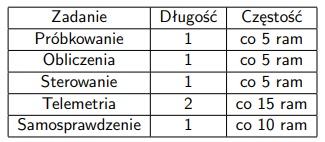
\includegraphics[scale=0.6]{rozdziały/images/SO/wymagania_czasowe.png}
        \end{minipage}\hfill
        \begin{minipage}{0.5\textwidth}
            \centering
            Tablica szeregująca
            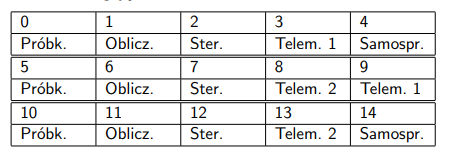
\includegraphics[scale=0.6]{rozdziały/images/SO/tablica_szeregujaca.png}
        \end{minipage}
    \end{figure}
    

    Istotne informacje:
    \begin{itemize}
        \item W sytuacji, w której zadanie nie mieści się w jednej ramie, trzeba podzielić je na części.
        \item Jeżeli zmieni się rozmiar ramy, to trzeba przeliczyć tablicę szeregującą i ponownie podzielić zadania na ramy.
        \item Jeśli zmieni się kod zadania, trzeba upewnić się że dalej mieście się w ramach.
        \item Jeśli zadanie nie wypełnia ramy - czas procesora się marnuje.
        \item Zastosowanie: systemy sterujące ze sztywnymi więzami czasowymi.
    \end{itemize}
    
    Wnioski:
    \begin{itemize}
        \item Zalety: powtarzalne, proste
        \item Wady: marnowanie czasu procesora, nieskalowalne, trudne w pielęgnacji
    \end{itemize}

\subsubsection{Szeregowanie asynchroniczne}   
    Klasyczne szeregowanie asynchroniczne, czyli takie w którym nie wiemy kiedy dokładnie wystąpi przełączenie kontekstu. Może być realizowane tak jak w systemach ogólnego przeznaczenia \textbf{z wywłaszczaniem} albo \textbf{bez wywłaszczania}. 

    Bez wywłaszczania:
    \begin{itemize}
        \item brak powtarzalności, zachowaniem terminów ostatecznych. Nie jesteśmy w stanie powiedzieć kiedy ostatecznie zakończy się zadanie, gdyż nie wiemy ile poprzednie będą się wykonywać.
    \end{itemize}

    Dlatego w praktyce stosuje się szeregowanie z wywłaszczaniem i priorytetami zadań.

\begin{problems}
    \prob Proces jest w stanie
    \answers{aktywnym, gdy jest obecnie wykonywany przez procesor}{wstrzymanym, gdy czeka na zakończenie operacji wejścia-wyjścia, lub czeka na jakieś zdarzenie}{gotowym, gdy zakończył się i czeka na odczytanie końcowego stanu przez rodzica}

    \prob W chwili $0$ w kolejce znajdują się procesy z następującą długością najbliższej fazy procesora: $$P = 10, \quad Q = 4, \quad R = 2, \quad S = 6$$
    \answers{w strategii szeregowania z podziałem czasu (ang. \textit{time sharing}) proces $R$ kończy swój ostatni przydział procesora w chwili $7$}{w strategii szeregowania rotacyjnego (ang. \textit{round-robin}) z kwantem czasu $3$ proces $Q$ kończy swój ostatni przydział procesora w chwili $15$}{w strategii szeregowania SJF (ang. \textit{shortest job first}) bez wywłaszczania proces $P$ dostaje procesor jako ostatni}
\end{problems}

\section{Zakleszczenia}

Zbiór procesów $P$ jest w stanie zakleszczenia, gdy każdy proces z $P$ czeka na zdarzenie, które może być spowodowane tylko przez inny proces z $P$.

\subsection{Warunki konieczne}
\begin{itemize}
    \item \textbf{niepodzielność} co najmniej jednego zasobu
    \item \textbf{przetrzymywanie} i \textbf{oczekiwanie} – pewien proces otrzymał co najmniej jeden zasób i oczekuje na inny przetrzymywany przez inny proces
    \item \textbf{brak wywłaszczeń} – zasób może być zwolniony jedynie dobrowolnie przez przetrzymujący go proces
    \item  \textbf{czekanie cykliczne} – istnieje zbiór procesów $\{P_0, \ldots, P_n\}$, taki że $P_i$ czeka na zasób przetrzymywany przez $P_{i+1}$ dla $i \in \{0, \ldots, n-1\}$, a $P_n$ czeka na zasób przetrzymywany przez $P_0$
\end{itemize}

\subsection{Graf przydziału zasobów}
To skierowany graf dwudzielny, którego wierzchołkami są:
\begin{itemize}
    \item procesy $P_1, P_2, \ldots$ - przedstawiane jako kółka
    \item zasoby systemu $Z_1, Z_2, \ldots$ - przedstawiane jako kwadraty
\end{itemize}
Ponadto:
\begin{itemize}
    \item Egzemplarze zasobów oznaczane są jako kropki
    \item Krawędź $P_i \xrightarrow{} Z_j$ oznacza, że $P_i$ zamówił $Z_j$ i czeka na niego
    \item Krawędź $Z_j \xrightarrow{} P_i$ oznacza, że $P_i$ ma przydzielony zasób $Z_j$
\end{itemize}

\begin{center}
            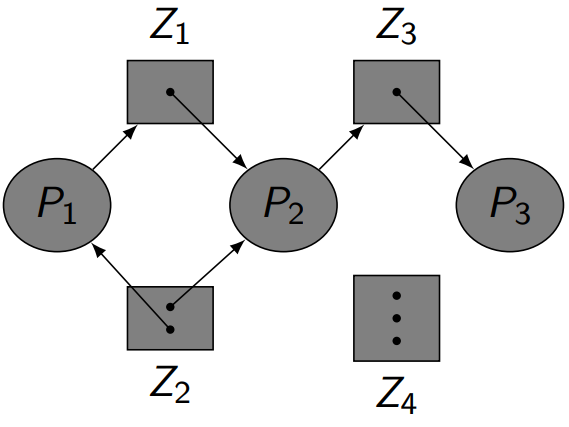
\includegraphics[scale=0.25]{rozdziały/images/SO/graf_przydzialu_zasobow.png}
\end{center}


\subsection{Warunek konieczny zakleszczenia}
Jeśli system jest w stanie zakleszczenia, to w grafie zasobów istnieje cykl.

\begin{center}
            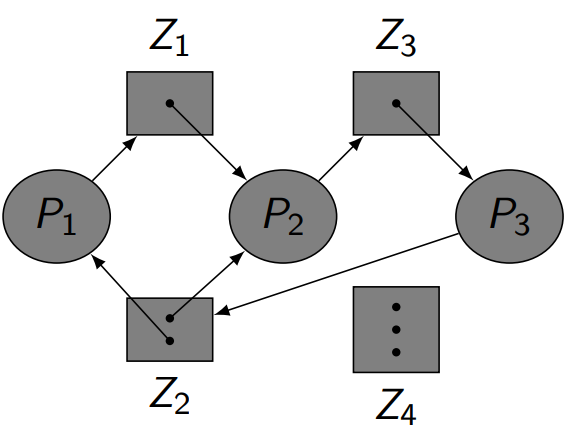
\includegraphics[scale=0.25]{rozdziały/images/SO/cykl_zakleszczenie.png}
    
\end{center}

Jednak odwrotne twierdzenie nie jest prawdziwe - kontrprzykład:

\begin{center}
            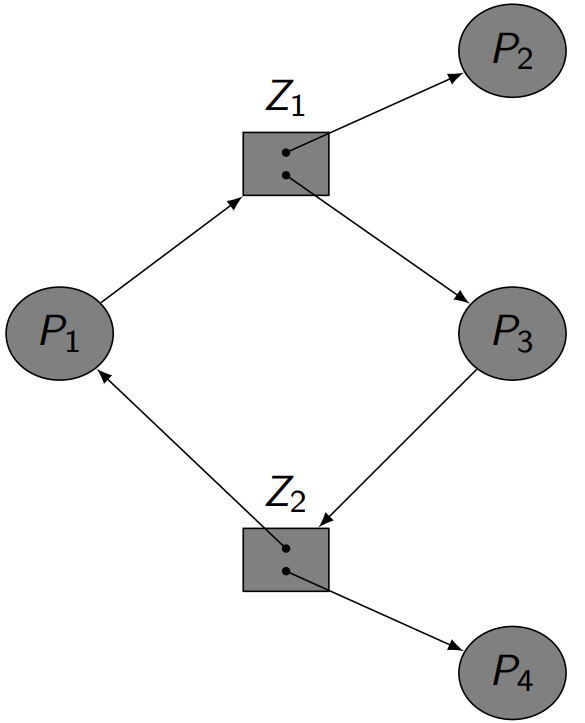
\includegraphics[scale=0.25]{rozdziały/images/SO/cykl_niezakleszczenie.png}
    
\end{center}


\subsection{Radzenie sobie z zakleszczeniami}

Można zapobiegać, unikać, wykrywać i usuwać lub nie robić nic. Nic nie robienie to najczęściej stosowane rozwiązanie we współczesnych systemach. \\\\ Jednak gdy zdecydujemy się co robić, to jak?

\begin{itemize}
    \item \textbf{Zapobieganie} -  upewnić się, że któryś z warunków koniecznych nie jest spełniony
    \item \textbf{Unikanie} - wprowadzamy pojęcia:
        \begin{itemize}
            \item Każdy proces deklaruje \textbf{maksymalną} liczbę potrzebnych zasobów każdego typu.
            \item \textbf{Stan bezpieczny} - stan, w którym system może przydzielić zasoby każdemu procesowi (w stopniu maksymalnym), unikając zakleszczenia. 
            \item \textbf{Stan zagrożenia} - stan, który nie jest bezpieczny. Stan zagrożenia może prowadzić do zakleszczenia.
            \item \textbf{Stan zakleszczenia} - szczególny przypadek stanu zagrożenia.
        \end{itemize}
        Następnie wykorzystujemy je przy realizacji algorytmu \textbf{Bankiera} - analogii bankiera, który nigdy nie zainwestuje gotówki w sposób uniemożliwiający zaspokojenie roszczeń wszystkich klientów
    \item \textbf{Wykrywanie} i \textbf{usuwanie}:
        \begin{itemize}
            \item Wykrywanie - symulacja przydziału i zwrotu zasobów na podstawie aktualnego stanu
            \item Usuwanie - kończenie procesów i wywłaszczanie zasobów
        \end{itemize}
\end{itemize}

\begin{problems}
    \prob W grafie przydziału zasobów istnieje cykl. Wynika z tego, że
    \answers{system jest w stanie blokady}{system jest w stanie bezpiecznym}{istnieje proces oczekujący na zasoby}
    
    \prob Warunkiem wystarczającym powstania zakleszczenia jest
    \answers
    {niepodzielność co najmniej jednego zasobu}
    {brak wywłaszczeń}
    {przetrzymywanie i oczekiwanie}
\end{problems}

\section{Zarządzanie pamięcią}
\textbf{Brak zarządzania pamięcią} -- użytkownik musi sam wszystko oprogramować.

\textbf{Pojedynczy obszar pamięci} -- pamięć użytkownika stanowi jeden duży obszar, system operacyjny udostępnia tylko podstawowe operacje (np ładowanie programów).

\textbf{Strefy statyczne} -- pamięć jest podzielona na pewną liczbę obszarów, każdy obszar ma ustalony rozmiar. W każdym obszarze może wykonywać się jeden proces. Gdy zgłasza się proces, szuka się dla niego wystarczająco dużego obszaru. Zachodzi \textbf{fragmentacja wewnętrzna} -- część obszaru przydzielonego pozostaje niewykorzystana.

\textbf{Przydział ciągły} --- procesy otrzymują ciągłe bloki pamięci. Obszary wolnej pamięci tworzą tzw. dziury. Gdy pojawia się proces, system operacyjny szuka dla niego wystarczająco obszernej dziury.
Zachodzi \textbf{fragmentacja zewnętrzna} -- suma rozmiarów wolnych obszarów by starczyła do spełnienia zamówienia, ale nie jest spójnym obszarem.

Przydział ciągły może być obsługiwany przez \textbf{algorytm bliźniaków}:
\begin{itemize}
    \vspace{-6pt} \item Pamięć jest podzielona na $2^n$ jednostek, początkowo stanowi jeden spójny blok. 
    \vspace{-6pt} \item Procesy zawsze proszą o $2^k$ jednostek (fragmentacja wewnętrzna). Jeśli nowy proces chce pamięć rozmiaru jakiegoś ciągłego bloku, to go dostaje. 
    \vspace{-6pt} \item W przeciwnym przypadku szukamy większego bloku i dzielimy go na pół, aż dojdziemy do oczekiwanego rozmiaru. 
    \vspace{-6pt} \item Przy oddawaniu pamięci, system operacyjny sprawdza, czy bliźniak bloku jest wolny. Jeśli tak, to sklejamy dopóki się da. 
\end{itemize}

\subsection{Stronicowanie}

Pamięć fizyczna jest podzielona na ramki o takim samym rozmiarze będącym potęgą dwójki, pamięć logiczna jest podzielona na strony o takim samym rozmiarze jak ramka.

Każdy proces ma tablicę stron, która zawiera odwzorowanie numerów stron na numery ramek

Wymaga wsparcia sprzętowego.

Adresy logiczne składają się z numeru strony i przesunięcia w obrębie strony.
\begin{example}
    W architekturze 32-bitowej przy rozmiarze strony 4 KiB:
    \begin{itemize}
        \vspace{-6pt} \item bity 0-11 oznaczają przesunięcie
        \vspace{-3pt} \item bity 12-31 oznaczają numer strony
    \end{itemize}
\end{example}

\begin{figure}[H]
    \centering
    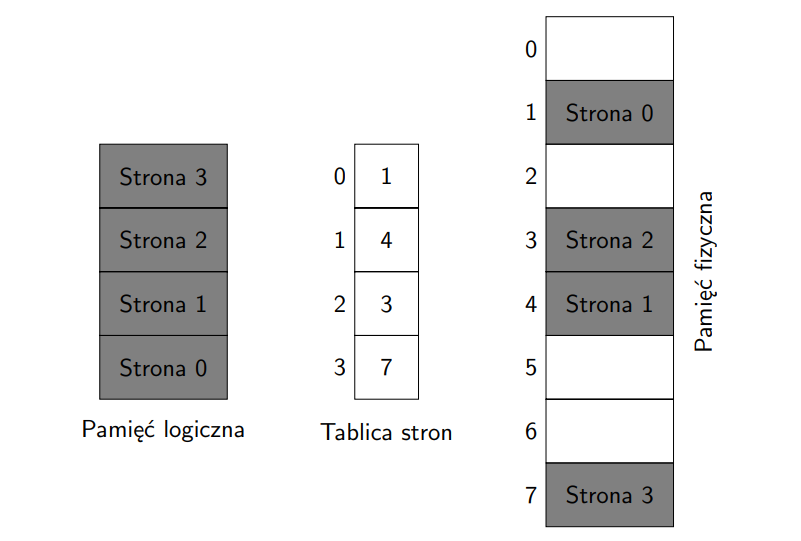
\includegraphics[scale=0.35]{rozdziały/images/SO/stronnicowanie.png}
    \caption{Przykład tablicy stron procesu}
\end{figure}

Translacja adresu jest wykonywana sprzętowo, polega na zamianie numeru strony na numer ramki, korzystając z tablicy stron.

Zalety: mała segmentacja wewnętrzna, brak segmentacji zewnętrznej.

Problemy:
\begin{itemize}
    \item Zwiększa się czas potrzebny na dostęp do komórki pamięci.

    Remedium: bufor translacji adresów strony (TLB). Mała, szybka pamięć asocjacyjna. Zawiera kilka pozycji z tablicy stron (pary numer strony, numer ramki).
    
    \item Tablica stron może być bardzo duża.

    Remedium: wielopoziomowe tablice stron.
    \begin{example}
        Przy dwupoziomowych tablicach stron, mamy katalog tablic stron który trzyma adresy odpowiednich tablic stron. Część komórek może być pusta, jeśli nie mamy odwołań do odpowiadającym ich adresom.

        Przy 32-bitowych adresach i rozmiarze strony 4KiB, przykładowy podział adresu:
        \begin{itemize}
            \vspace{-3pt} \item bity 0-11 oznaczają przesunięcie
            \vspace{-3pt} \item bity 12-21 oznaczają indeks w tablicy stron
            \vspace{-3pt} \item bity 22-31 oznaczają indeks w katalogu tablic stron
        \end{itemize}
    \end{example}
\end{itemize}

\subsection{Pamięć wirtualna}
Przy \textbf{pamięci wirtualnej}, nie wszystkie strony procesu muszą być w pamięci fizycznej.

W tablicy stron przechowywany jest bit, który informuje, czy dana strona znajduje się w pamięci operacyjnej. 
Gdy następuję odwołanie do niezaładowanej strony, sprzęt stronicujący wykrywa nieustawiony bit i generuje błąd braku strony.

System operacyjny obsługuje błąd braku strony. Sprawdzane jest, czy odwołanie jest dozwolone, po czym znajdowana jest wolna ramka i ewentualne następuje sprowadzenie strony z dysku.

\begin{exam}
    W systemie z wirtualną pamięcią i stronicowaniem strona ma rozmiar 2MiB, adres wirtualny -- 48 bitów, adres fizyczny -- 40 bitów. Wtedy w systemie mogą istnieć
    \answers
    {proces z adresem wirtualnym \texttt{0x00c00f04} zmapowanym na adres \texttt{0x00d00004}}
    {proces z adresem wirtualnym \texttt{0x0a000004} zmapowanym na adres \texttt{0x00800004}}
    {proces z adresem wirtualnym \texttt{0x000c0000} oraz proces z adresem wirtualnym \texttt{0x001a0000} zmapowanymi na ten sam adres fizyczny \texttt{0x00140000}}

    Strona ma rozmiar 2MiB, zatem offset będzie miał $21$ bitów (1MiB to $2^{20}$ bajtów).

    A. Adres wirtualny \texttt{0x00c00f04} ma offset \texttt{0x000f04}, adres fizyczny ma \texttt{0x00d00004} ma offset \texttt{0x100004}, zatem takie mapowanie jest niepoprawne

    B. Adres wirtualny \texttt{0x0a000004} ma offset \texttt{0x000004}, adres fizyczny \texttt{0x00800004} ma offset \texttt{0x000004}, zatem takie mapowanie mogło by się wydarzyć.

    C. Nie, bo offsety się nie zgadzają. (Gdyby się zgadzały, to
    taka sytuacja jest możliwa, na przykład po wywołaniu {\ttfamily fork()}))
\end{exam}

\begin{problems}
    \prob Fragmentacja wewnętrzna pamięci
    \answers{może wystąpić przy zarządzaniu pamięcią metodą stronicowania}{polega na tym, że część obszaru przydzielonego procesowi pozostaje niewykorzystana}{może wystąpić przy zarządzaniu pamięcią metodą stref statycznych}

    \prob Fragmentacja wewnętrzna to
    \answers{niemożność przydziału procesowi spójnego kawałka pamięci pomimo posiadania wystarczającej ilości pamięci}{występowanie bezużytecznych obszarów pamięci w pamięci procesu}{niemożność scalenia wielu małych bloków pamięci w jeden duży}

    \prob Tablica stron
    \answers{zawiera informacje o rozmieszczeniu stron procesu w pamięci fizycznej}{jest tworzona podczas kompilacji programu}{jest wykorzystywana podczas translacji adresów}

    \prob Bufory translacji adresów (TLB)
    \answers
    {przechowują dane z tych komórek pamięci, do których procesor odwoływał się niedawno}
    {redukują liczbę odwołań do tablic stron}
    {mogą być realizowane w postaci szybkiej pamięci asocjacyjnej}

    \prob W pewnym systemie operacyjnym z wirtualizacją pamięci strona ma rozmiar 8KiB, adres wirtualny jest 56-bitowy, a adres fizyczny jest 44-bitowy. Istnieje taka konfiguracja mapowania adresów dwóch różnych procesów $A$ i $B$, że
    \answers{adres wirtualny $(123456)_{16}$ procesu $A$ jest odwzorowywany na adres fizyczny $(312456)_{16}$}{adres wirtualny $(123456)_{16}$ procesu $B$ jest odwzorowywany na adres fizyczny $(321456)_{16}$}{zarówno adres wirtualny $(\text{abcdef})_{16}$  procesu $A$, jak i adres wirtualny $(\text{abcdef})_{16}$ procesu $B$ są odwzorowywane na ten sam adres fizyczny $(\text{abcdef})_{16}$}
    
    \prob Mamy proces z 52-bitową pamięcią wirtualną i 48-bitową pamięcią fizyczną. Zastosowane jest stronicowanie dwupoziomowe, a wielkość wpisu w tablicy stron i katalogu tablic stron wynosi 16B. Wówczas
    \answers{strona ma 16 KiB}{numer strony ma 16 bitów}{istnieje konfiguracja, która adresowi fizycznemu 0x16161616 przypisuje adres wirtualny 0x61611616}
    
    \prob Pewien procesor używa jednopoziomowego mechanizmu stronicowania. Rozmiar tablicy stron jest równy rozmiarowi strony. Jeden wpis w tablicy stron zajmuje 4 bajty. Adres wirtualny ma 32 bity. Wynika z~tego, że w tym procesorze
    \answers{strona ma rozmiar 4 KiB}{górne ograniczenie na rozmiar pamięci fizycznej wynosi 4 GiB}{procesowi można przydzielić co najwyżej 32768 stron}
    
    \prob W pewnym systemie operacyjnym, w którym zaimplementowano stronicowanie, rozmiar strony wynosi 1 kilobajt. Tablica stron każdego procesu mieści się na jednej stronie, a każdy wpis w tablicy stron zajmuje 2 bajty. Wynika z tego, że:
    \answers{pamięć operacyjna jest nie większa niż 512 kilobajtów}{przestrzeń adresowa procesu jest nie większa niż 512 kilobajtów}{przestrzeń adresowa procesu jest nie większa niż 512 bajtów}

    \prob Pamięć ze spójnego obszaru o wielkości $1$ MiB jest przydzielana metodą bliźniaków. Cztery procesy kolejno poprosiły o przydział pamięci o wielkości: $32$ KiB, $256$ KiB, $512$ KiB i $64$ KiB. W wyniku przetworzenia tej sekwencji żądań
    \answers{każdy proces otrzymał spójny obszar pamięci}{wszystkie żądania zostały spełnione}{największe żądanie, które może teraz zostać spełniona, to prośba o przydział pamięci wielkości $128$ KiB}

    \prob W pewnym systemie komputerowym, w którym zastosowano dwupoziomowe stronicowanie, adresy logiczne są 48-bitowe, rozmiar strony, katalogu tablic stron i tablicy stron mają 256 KiB, a wpis w katalogu i tablicy zajmuje 8B. Wówczas
    \answers{offset ma 17 bitów}{numer strony ma 16 bitów}{numer tablicy stron ma 15 bitów}
    
    \prob W pewnym systemie komputerowym, w którym zastosowano stronicowanie, odwołania do pamięci generowane przez procesy są 16-bitowe. Rozmiar strony wynosi 1 KiB (1024 bajty), a jeden wpis w tablicy stron zajmuje 2 bajty. Wynika z tego, że
    \answers
    {tablica stron mieści się na jednej stronie}
    {proces może zaadresować przestrzeń wielkości 512 KiB}
    {tablica stron musi być co najmniej dwupoziomowa}
\end{problems}

\section{System plików}

\textbf{Plik} -- logiczny pojemnik na dane. System operacyjny udostępnia pewne operacje do zarządzania plikami, ale nie interpretuje ich zawartości, traktując go jako ciąg bajtów.

Dowiązanie -- odniesienie pliku do katalogu. Do jednego pliku może istnieć wiele dowiązań.

Informacje o pliku, takie jak liczba dowiązań i położenie bloków z danymi, są przechowywane na dysku w \textbf{i-węźle}.

Przed użyciem plik należy otworzyć. Funkcja systemowa open pobiera jako argument nazwę ścieżkową pliku, a przekazuje w wyniku \textbf{deskryptor}.
Deskryptor pliku można traktować jako sesję dostępu do pliku. 

Deskryptory mogą być duplikowane, na przykład przez wywołanie {\ttfamily fork()}
Wielokrotne otwieranie tego samego pliku tworzy nowe deskryptory.

W strukturze danych procesów znajdują się tablica z informacjami o otwartych przez proces plikach, której komórki odpowiadają kolejnym deskryptorom. Znajdują tam się odniesienia do systemowej tablicy otwartych plików. 

Wywołanie `open()` tworzy nową pozycję w systemowej tablicy otwartych plików, ale `fork()` tylko zwiększa liczbę odniesień do jednej pozycji w tablicy.

\subsection{ext2}

\textbf{ext2} to jedna z implementacji systemu plików. 

Przy inicjowanie systemu administrator wybiera optymalny rozmiar \textbf{bloku} (zazwyczaj 1-4 KiB) oraz liczbę i-węzłów dla partycji określonego rozmiaru. 

Pierwszy blok partycji jest zarezerwowany dla sektora startowego. Reszta partycji jest podzielona na \textbf{grupy bloków}. Mapa bitowa opisująca stan zajętości bloków w grupie musi się mieścić w jednym bloku.

\begin{example}
    Jeśli plik ma rozmiar 1KiB, to grupa może mieć rozmiar 8MiB, ponieważ bitmapa bloków posiada $8 \cdot 1024$
    bitów, więc w grupie zmieści się $8 \cdot 1024$ bloków po 1KiB każdy.
\end{example}

Maksymalny rozmiar pliku to:
$$\text{min} \left( 
    \left( \frac{b}{4} \right)^3 +
    \left( \frac{b}{4} \right)^2 +
    \left( \frac{b}{4} \right) + 12, 2^{41} \right)
$$
gdzie $b$ to chyba rozmiar pliku. Dowód pozostawiamy jako ćwiczenie dla czytelnika.

Maksymalny rozmiar partycji zależy od $32$-bitowych numerów bloków na dysku, czyli jest to $2^{32} \cdot$ {\ttfamily rozmiar\_bloku}.

\begin{solutions}
% ASM
    % Grześ
    \sol W procesorze x86 wykonano następujące instrukcje:
    \begin{gas}
        mov al, 3
        mov bl, 130
        sub al, bl
    \end{gas}
    Wtedy
    \answerss{w rejestrze \gasinline{al} jest zapisana wartość $-127$ przy interpretacji w kodzie uzupełnień do dwóch}{w rejestrze \gasinline{al} jest zapisana wartość $127$ przy interpretacji w naturalnym kodzie binarnym}{ustawione zostaną flagi CF, OF, SF}{TAK}{NIE}{TAK}
    \textbf{A.} W U2 pod \gasinline{al} zapisane jest 3, pod \gasinline{bl} -126, więc po odjęciu dostaniemy 129, czyli $-127$ w U2.

    \textbf{B.} w NKB pod \gasinline{al} zapisane jest 3, pod \gasinline{bl} 130, więc po odjęciu dostajemy $-127$, co przeskoczy na 129 w NKB.

    \textbf{C.} Flaga CF zostanie ustawiona, ponieważ wynik operacji $-127$ nie mieści się w zakresie NKB. Flaga OF również zostanie ustawiona, bo przy interpretacji U2 rejestr \gasinline{bl} przechowuje wartość $-126$, więc wynikiem operacji będzie 129, co jest spoza zakresu U2 i zostanie przekonwertowane na $-127$. Flaga SF również zostanie ustawiona, ponieważ jak widzimy, wynikiem operacji jest liczba ujemna, więc pierwszy bit wyniku w interpretacji U2 ustawiony jest na 1.

    % Julia
    \sol Cechą architektury RISC jest
    \answerss{zapisywanie wyników instrukcji arytmetyczno-logicznych tylko w rejestrach}{kodowanie wszystkich instrukcji maszynowych za pomocą tej samej liczby bajtów}{dopuszczenie adresowania niewyrównanego}{TAK}{TAK}{NIE}
    Odpowiedzi z tabelki wyżej

    % Julia
    \sol Cechą architektury CISC jest
    \answerss
    {zapisywanie wyników instrukcji arytmetyczno-logicznych tylko w rejestrach}
    {kodowanie wszystkich instrukcji maszynowych za pomocą tej samej liczby bajtów}
    {dopuszczenie adresowania niewyrównanego}
    {NIE}{NIE}{TAK}
    Odpowiedzi z tabelki wyżej

    % Wiktor
    \sol W czterech kolejnych bajtach pamięci, począwszy od adresu $X$, znajdują się odpowiednio wartości 1, 3, 5 i 7. Procesor cienkokońcówkowy (ang. \textit{little-endian}) wczytał 32-bitową liczbę spod adresu $X$, odjął od niej $(16)_{10}$ i zapisał wynik pod adresem $X$. Po tych operacjach bajt o adresie
    \answerss{$X$ zawiera wartość $(F1)_{16}$}{$X+1$ zawiera wartość $(03)_{16}$}{$X+2$ zawiera wartość $(05)_{16}$}{TAK}{NIE}{TAK}
    Mamy do czynienia z procesorem cienkokońcówkowym, czyli najmniej znaczące bity są zapisane na początku. Liczba pod $X$ to $1\cdot 2^0 + 3 \cdot 2^8 + 5\cdot 2^{16} + 7\cdot 2^{24}$ i odejmujemy $16$. Wystarczy spojrzeć na adresy $X$ i $X+1$. Pod nimi otrzymamy $1 + 3\cdot 256 - 16= 769-16=753$. $\floor{\frac{753}{256}}=2$. Pod $X+1$ mamy liczbę $2$, a pod $X$ mamy $753-2\cdot 256=241 = (F1)_{16}$. Stąd \textbf{A.} to prawda, a \textbf{B.} to nieprawda.
    \textbf{C.} adres $X+2$ nie zostanie tknięty, nadal jest ta sama wartość co przed odejmowaniem.

    % Julia
    \sol W ośmiobitowym rejestrze procesora zapisana jest wartość $(10101100)_2$, która interpretowana
    \answerss{w naturalnym kodzie binarnym reprezentuje liczbę 162}{w kodzie uzupełnieniowym do dwójki reprezentuje liczbę $-84$}{w kodzie moduł-znak reprezentuje liczbę $-43$}{NIE}{TAK}{NIE}
    \textbf{A.} Liczby w naturalnym kodzie binarnym są interpretowane jako: $\sum_{i = 0}^{n - 1} b_i 2^i$, zatem wartość z polecenia to będzie $2^7+2^5+2^3+2^2=172$ \\
    \textbf{B.} Liczby w kodzie uzupełnieniowym do dwójki są interpretowane jako: $-b_{n-1} 2^{n - 1} + \sum_{i = 0}^{n - 2} b_i 2^i$, zatem wartość z polecenia to będzie $-2^7+2^5+2^3+2^2=-84$ \\
    \textbf{C.} Liczby w kodzie moduł-znak są interpretowane jako: $(-1)^{b_{n-1}} \cdot \sum_{i = 0}^{n - 2} b_i 2^i$, zatem wartość z polecenia to będzie $(-1) \cdot (2^5+2^3+2^2) = -44$

    \sol Przetwarzanie potokowe
    \answerss{zawsze przyspiesza lub nie spowalnia wykonywania rozkazów}{niewykorzystywane jest dla rozkazu skoku}{zostało zastosowane po raz pierwszy w procesorach Pentium}{TAK}{NIE}{NIE}
    \textbf{A.} IMO kontrowersyjne, bo jednak stosowane jest tłumaczenie rozkazów z CISC na RISC, co zajmuje jakiś czas i może być pechowy case samych jumpów itd., ale niech będzie, że ogólnie przyspiesza.
    
    \textbf{B.} Wykorzystuje się, choć są problematyczne. Dziś korzysta się też z tzw. predykcji skoków.
    
    \textbf{C.} Bez komentarza.

    \sol Każdy procesor 32-bitowy ma
    \answerss
    {32-bitową zewnętrzną szynę danych}
    {32-bitową zewnętrzną szynę adresową}
    {32-bitowe rejestry danych}
    {NIE}{NIE}{TAK}
    
% szeregowanie
    % Grześ
    \sol Proces jest w stanie
    \answerss{aktywnym, gdy jest obecnie wykonywany przez procesor}{wstrzymanym, gdy czeka na zakończenie operacji wejścia-wyjścia, lub czeka na jakieś zdarzenie}{gotowym, gdy zakończył się i czeka na odczytanie końcowego stanu przez rodzica}{TAK}{TAK}{NIE}
    \textbf{A.} i \textbf{B.} z definicji. \textbf{C.} opisuje proces w stanie ,,zakończony".

    % Jasiek
    \sol W chwili $0$ w kolejce znajdują się procesy z następującą długością najbliższej fazy procesora: $$P = 10, \quad Q = 4, \quad R = 2, \quad S = 6$$
    \answerss{w strategii szeregowania z podziałem czasu (ang. \textit{time sharing}) proces $R$ kończy swój ostatni przydział procesora w chwili $7$}{w strategii szeregowania rotacyjnego (ang. \textit{round-robin}) z kwantem czasu $3$ proces $Q$ kończy swój ostatni przydział procesora w chwili $15$}{w strategii szeregowania SJF (ang. \textit{shortest job first}) bez wywłaszczania proces $P$ dostaje procesor jako ostatni}{NIE}{TAK}{TAK}

    \textbf{A.} Time sharing jest tak naprawdę round-robinem z epsilonowym kwantem czasu. Z tego powodu proces $R$ kończy swój ostatni przydział procesora w chwili $4 \cdot 2 = 8$.

    \textbf{B.} Procesy używają procesora w następującej kolejności:
    \begin{itemize}
        \item $P$ używa procesora przez 3 kwanty czasu;
        \item $Q$ używa procesora przez 3 kwanty czasu;
        \item $R$ używa procesora przez 2 kwanty czasu (i kończy się);
        \item $S$ używa procesora przez 3 kwanty czasu;
        \item $P$ używa procesora przez 3 kwanty czasu;
        \item $Q$ używa procesora przez 1 kwant czasu (i kończy się).
    \end{itemize}

    \textbf{C.} Z definicji SJF $P$ jako proces zajmujący procesor na najdłużej wykona się jako ostatni.

% zasoby
    % Grześ
    \sol W grafie przydziału zasobów istnieje cykl. Wynika z tego, że
    \answerss{system jest w stanie blokady}{system jest w stanie bezpiecznym}{istnieje proces oczekujący na zasoby}{NIE}{NIE}{TAK}
    \textbf{A.} To, że istnieje cykl, nie znaczy, że mamy zakleszczenie (patrz: rysunek przy warunkach koniecznych zakleszczenia).

    \textbf{B.} To, że mamy cykl, \textbf{może} znaczyć, że jest zakleszczenie, a to z pewnością nie jest stan bezpieczny.

    \textbf{C.} Gdyby nikt nie czekał na zasoby, to cykl nie jest możliwy.

    % Patryk
    \sol Warunkiem wystarczającym powstania zakleszczenia jest
    \answerss
    {niepodzielność co najmniej jednego zasobu}
    {brak wywłaszczeń}
    {przetrzymywanie i oczekiwanie}
    {NIE}{NIE}{NIE}
    
    Wszystkie te warunki są warunkami koniecznymi, ale żaden z nich nie jest wystarczający.

% pamięć
    % Grześ
    \sol Fragmentacja wewnętrzna pamięci
    \answerss{może wystąpić przy zarządzaniu pamięcią metodą stronicowania}{polega na tym, że część obszaru przydzielonego procesowi pozostaje niewykorzystana}{może wystąpić przy zarządzaniu pamięcią metodą stref statycznych}{TAK}{TAK}{TAK}
    \textbf{A.} Niewielka, ale występuje.

    \textbf{B.} Dokładnie tak.

    \textbf{C.} Występuje, i to w większym stopniu niż przy stronicowaniu.

    % Grześ
    \sol Fragmentacja wewnętrzna to
    \answerss{niemożność przydziału procesowi spójnego kawałka pamięci pomimo posiadania wystarczającej ilości pamięci}{występowanie bezużytecznych obszarów pamięci w pamięci procesu}{niemożność scalenia wielu małych bloków pamięci w jeden duży}{NIE}{TAK}{NIE}
    \textbf{A.} Jest to definicja fragmentacji zewnętrznej.

    \textbf{B.} Taka jest właśnie definicja.

    \textbf{C.} Nie jest to fragmentacja wewnętrzna, tylko przykład patologii w algorytmie bliźniaków.

    \sol Tablica stron
    \answerss{zawiera informacje o rozmieszczeniu stron procesu w pamięci fizycznej}{jest tworzona podczas kompilacji programu}{jest wykorzystywana podczas translacji adresów}{TAK}{NIE}{TAK}
    \textbf{A.} Z definicji tym się zajmuje, tak samo \textbf{C.} Skoro każdy proces ma swoją tablicę stron, to ciężko, żeby była ona tworzona w czasie kompilacji programu, kiedy nie wiadomo ile procesów w trakcie powstanie, zatem \textbf{B.} to nieprawda.
    
    % Wiktor
    \sol Bufory translacji adresów (TLB)
    \answerss
    {przechowują dane z tych komórek pamięci, do których procesor odwoływał się niedawno}
    {redukują liczbę odwołań do tablic stron}
    {mogą być realizowane w postaci szybkiej pamięci asocjacyjnej}
    {NIE}{TAK}{TAK}
    \textbf{A.} Nie, nie zawiera danych z tych komórek pamięci (to by zajmowało bardzo dużo pamięci, a TLB są bardzo małe). Zawiera jedynie informacje gdzie te dane są, redukując potrzebę odwoływania się do tablicy stron. Stąd \textbf{B.} to prawda. \textbf{C.} tak po prostu jest.

    % Grześ
    \sol W pewnym systemie operacyjnym z wirtualizacją pamięci strona ma rozmiar 8KiB, adres wirtualny jest 56-bitowy, a adres fizyczny jest 44-bitowy. Istnieje taka konfiguracja mapowania adresów dwóch różnych procesów $A$ i $B$, że
    \answerss{adres wirtualny $(123456)_{16}$ procesu $A$ jest odwzorowywany na adres fizyczny $(312456)_{16}$}{adres wirtualny $(123456)_{16}$ procesu $B$ jest odwzorowywany na adres fizyczny $(321456)_{16}$}{zarówno adres wirtualny $(\text{abcdef})_{16}$  procesu $A$, jak i adres wirtualny $(\text{abcdef})_{16}$ procesu $B$ są odwzorowywane na ten sam adres fizyczny $(\text{abcdef})_{16}$}{NIE}{TAK}{TAK}
    Strona ma rozmiar 8KiB, czyli $2^{13}$B. Oznacza to, że offset ma 13 bitów. Do zweryfikowania odpowiedzi będziemy liczyć offsety adresu wirtualnego i fizycznego, czyli najmłodsze 13 bitów adresów.
    
    \textbf{A.} Offset adresu wirtualnego to $(1456)_{16}$, a fizycznego $(0456)_{16}$, więc takie mapowanie jest niemożliwe.

    \textbf{B.} Offset adresu wirtualnego to $(1456)_{16}$, a fizycznego $(1456)_{16}$. Są równe, więc takie mapowanie jest możliwe.

    \textbf{C.} Każdy proces ma swoją osobną tablicę stron, a offsety wszystkich wymienionych tu adresów są sobie równe. Jednakże, dwa różne procesy nie mogą wskazywać na ten sam adres fizyczne, ale taka sytuacja może się wydarzyć po wywołaniu \texttt{fork()}.

    % Patryk
    \sol Mamy proces z 52-bitową pamięcią wirtualną i 48-bitową pamięcią fizyczną. Zastosowane jest stronicowanie dwupoziomowe, a wielkość wpisu w tablicy stron i katalogu tablic stron wynosi 16B. Wówczas
    \answerss{strona ma 16 KiB}{numer strony ma 16 bitów}{istnieje konfiguracja, która adresowi fizycznemu 0x16161616 przypisuje adres wirtualny 0x61611616}{NIE}{TAK}{NIE}

    \textbf{A.} Załóżmy że strona ma rozmiar $S = 2^kB$. Wobec tego wpisów w tablicy jest $\frac{2^k}{2^4}$, tak samo w katalogu tablic. Różnych stron może być tyle ile jest wpisów więc jest to $\frac{S^2}{2^8}$. Żeby je zakodować potrzebujemy $\log(\frac{2^{2k}}{2^8}) = 2k - 8$. Dodatkowo skoro strona mieści $2^k B$ to potrzebujemy $k$ bitów (offset) żeby mieć dostęp do konkretnego bajtu w stronie. Otrzymujemy więc równość $2k - 8 + k = 52 \implies k = 20$. Zatem strona ma rozmiar $2^{20}B$ czyli 1MiB.

    \textbf{B.} Skoro strona ma $2^20$ B a wpis zajmuje $2^4B$ to stron jest $2^16$ wiec numer strony zawiera 16 bitów.

    \textbf{C.} 20 bitów na offset to 5 ostatnich znaków. Widzimy że 5 bit od końca różni się w obu tych adresach więc NIE.

    % Patryk
    \sol Pewien procesor używa jednopoziomowego mechanizmu stronicowania. Rozmiar tablicy stron jest równy rozmiarowi strony. Jeden wpis w tablicy stron zajmuje 4 bajty. Adres wirtualny ma 32 bity. Wynika z~tego, że w tym procesorze
    \answerss{strona ma rozmiar 4 KiB}{górne ograniczenie na rozmiar pamięci fizycznej wynosi 4 GiB}{procesowi można przydzielić co najwyżej 32768 stron}{NIE}{NIE}{TAK}

    \textbf{A.} Załóżmy że strona ma rozmiar $S = 2^kB$. Wobec tego wpisów w tablicy jest $\frac{2^k}{4}$. Różnych stron może być tyle ile jest wpisów, a żeby je zakodować potrzebujemy $\log(\frac{2^k}{4}) = k - 2$ bitów. Dodatkowo, skoro strona mieści $2^k B$ to potrzebujemy $k$ bitów (offset), żeby mieć dostęp do konkretnego bajtu w stronie. Otrzymujemy więc równość $k - 2 + k = 32 \implies k = 17$. Zatem strona ma rozmiar $2^{17}B$ czyli 128 KiB. 

    \textbf{B.} Pamięć fizyczna może przekroczyć 4 GiB, patrz: \href{https://pl.m.wikipedia.org/wiki/Physical_Address_Extension}{link}.
    
    \textbf{C.} Wpisów jest $2^{15} = 32768$, więc tyle można przydzielić stron procesowi.
    
    \sol W pewnym systemie operacyjnym, w którym zaimplementowano stronicowanie, rozmiar strony wynosi 1 kilobajt. Tablica stron każdego procesu mieści się na jednej stronie, a każdy wpis w tablicy stron zajmuje 2 bajty. Wynika z tego, że:
    \answerss{pamięć operacyjna jest nie większa niż 512 kilobajtów}{przestrzeń adresowa procesu jest nie większa niż 512 kilobajtów}{przestrzeń adresowa procesu jest nie większa niż 512 bajtów}{NIE}{TAK}{NIE}

    % Jasiek
    \sol Pamięć ze spójnego obszaru o wielkości $1$ MiB jest przydzielana metodą bliźniaków. Cztery procesy kolejno poprosiły o przydział pamięci o wielkości: $32$ KiB, $256$ KiB, $512$ KiB i $64$ KiB. W wyniku przetworzenia tej sekwencji żądań
    \answerss{każdy proces otrzymał spójny obszar pamięci}{wszystkie żądania zostały spełnione}{największe żądanie, które może teraz zostać spełniona, to prośba o przydział pamięci wielkości $128$ KiB}{TAK}{TAK}{TAK}

    Z definicji metody \href{https://ocdn.eu/images/pulscms/NzQ7MDA_/c7e85be71d20e087115f0d8465fea342.jpg}{bliźniaków} wiemy, że po prośbie pierwszego procesu struktura pamięci będzie wyglądała tak:
    \begin{center}
        \begin{tabular}{ | c | c | c | c | c | c | } 
            \hline
            32 KiB & 32 KiB & 64 KiB & 128 KiB & 256 KiB & 512 KiB \\
            \hline
        \end{tabular}
    \end{center}
    Zatem przychodzące procesy otrzymają kolejno pierwszy, piąty, szósty oraz trzeci fragment pamięci. Czwarty fragment pozostał niewykorzystany. Zatem wszystkie odpowiedzi to TAK.

    % Grześ
    \sol W pewnym systemie komputerowym, w którym zastosowano dwupoziomowe stronicowanie, adresy logiczne są 48-bitowe, rozmiar strony, katalogu tablic stron i tablicy stron mają 256 KiB, a wpis w katalogu i tablicy zajmuje 8B. Wówczas
    \answerss{offset ma 17 bitów}{numer strony ma 16 bitów}{numer tablicy stron ma 15 bitów}{NIE}{NIE}{TAK}
    \textbf{A.} Rozmiar strony to 256 KiB, więc $2^18$ B. Znaczy to, że offset ma 18 bitów.

    \textbf{B.} Skoro offset ma 18 bitów, a adres logiczny 48, to numer strony ma połowę pozostałych bitów, czyli $(48-18)/2=15$.

    \textbf{C.} Jest to 15 bitów, tyle samo co numer strony.

    % Patryk
    \sol W pewnym systemie komputerowym, w którym zastosowano stronicowanie, odwołania do pamięci generowane przez procesy są 16-bitowe. Rozmiar strony wynosi 1 KiB (1024 bajty), a jeden wpis w tablicy stron zajmuje 2 bajty. Wynika z tego, że
    \answerss
    {tablica stron mieści się na jednej stronie}
    {proces może zaadresować przestrzeń wielkości 512 KiB}
    {tablica stron musi być co najmniej dwupoziomowa}
    {TAK}{NIE}{NIE}

    \textbf{A.} Mamy do dyspozycji 16 bitów. Tablica ma $2^{10}B = 1024B$ więc offset zajmuje 10 bitów. Zatem zostaje 6 bitów na tablicę stron, jeden wpis zajmuje 2B więc będzie $2^5 = 32$ wpisów o wielkości 2B, więc spokojnie się zmieści na jednej stronie.

    % TODO: sprawdzić poprawność rozwiązania do podpunktu A. i ew. poprawić
    \textbf{\red{Przyp. red.: powyższe rozumowanie jest potencjalnie błędne: 6 bitów na tablicę stron oznacza 6 bitów na indeks w tablicy stron, tj. stron może być 64 (rozmiar wpisu nie ma tu nic do rzeczy)}}

    \textbf{B.} Skoro do dyspozycji jest 16 bitów, to może zaadresować max $2^{16} = 64$ KiB.

    \textbf{C.} Skoro tablica stron mieści się na jednej stronie to nie musi być dwupoziomowa.
\end{solutions}
